   
\documentclass[11pt]{article}
\usepackage{amsmath,amsthm,verbatim,amssymb,amsfonts,amscd, graphicx}
\usepackage{graphicx}
\usepackage{listings}
\usepackage{float}
\usepackage{url}
\graphicspath{{./times/}}
\topmargin0.0cm
\headheight0.0cm
\headsep0.0cm
\oddsidemargin0.0cm
\textheight23.0cm
\textwidth16.5cm
\footskip1.0cm

\begin{document}
\title{CS 5220\\ Project 2 - Shallow Water Simulation}
\author{Marc Aurele Gilles (mtg79)\\ Sheroze Sheriffdeen(mss385)}
\maketitle

\section{Introduction}
Define structured grid computations \\
Define shallow water simulations \\
Math overview and associated abstractions in code\\

\section{Design Decisions}

The following sections describe the implementation changes from the original code found at \url{https://github.com/cornell-cs5220-f15/water}.

\subsection{Memory Layout}
The original solution a two dimensional vectors of 3-vectors to represent $U_t$, $F(U)_x$, and $G(U)_y$. During each time step, the solution accesses each element in the 2-D grid sequentially. Then, the \texttt{vector<vector<real>>} representation leads to memory accesses that are not local spatially. \\

Therefore, our solution chooses to use 3 separate two dimensional vectors per objects, $U_t$, $F(U)_x$, and $G(U)_y$. Thus, we are required in general to perform three loop iterations in place of a single loop in the original solution. But this approach leverages spatial locality, especially in \texttt{compute\_step} and \texttt{limited\_derivs} functions.

\subsection{Vectorization}

By observing the profiling information, we noticed that the original solution spends majority of its computational time in the functions \texttt{limited\_derivs}, \texttt{compute\_step} and \texttt{compute\_fg\_speeds}. By adopting the newer memory layout, we enabled spatially local memory accesses. We were also able to decompose \texttt{for} loops in the solution to improve vectorization. Refer to \texttt{ipo\_out\_vectorization.optrpt} in \url{https://github.com/sheroze1123/water/tree/vectorization} for more information. \\

In \texttt{compute\_fg\_speeds}, we performed two separate loops to compute flux and wave speeds. The flux computation and the wave speed computation for the complete grid is not handled by the \texttt{Physics} class. We used \texttt{\#pragma simd} directives to instruct the compiler the ability to vectorize these computations. The compiler was successfully able to vectorize these functions with an estimated potential speedup of 6.7. \\

\texttt{limited\_derivs} uses the \texttt{limdiff} function in \texttt{minmod.h}. To improve the vectorization of this computation, we changed the implementation of \texttt{limdiff} in the following ways. 

\begin{enumerate}
	\item \texttt{limdiff} now performs the computation on the complete grid instead of at one grid point.
	\item \texttt{limdiff} was decomposed as \texttt{limdiff\_x} and \texttt{limdiff\_y} to perform the limiter along the $x$ dimension and the $y$ dimension separately while still retaining unit stride. 
\end{enumerate}

\subsection{Parallelization}
The updated memory layout is amenable to parallelization via OpenMP, particular during the costly operations of \texttt{limited\_derivs} and \texttt{compute\_step}. \\

At the beginning of a call to \texttt{limited\_derivs} we initialize a team of threads using \texttt{\#pragma omp parallel}. Each application of the limiter to the components of $U_t$, $F(U)_x$, and $G(U)_y$ can be computed in parallel since we removed the data dependencies by creating 3 separate two dimensional arrays per component. We use the \texttt{\#pragma omp for} directive to parallelize the grid computation of each component. \\

In \texttt{compute\_step}, we initialize a team of threads using \texttt{\#pragma omp parallel}. The predictor step is now performed in parallel. Then, we create a barrier before proceeding to the corrector step since the the corrector step needs information from the predictor. After computing the corrector step, we perform a barrier before finally copying back to storage in parallel. The performance increase we observed via parallelization reached up to 3+ speedup. Results are plotted in section~\ref{sec:speedup}.


\subsection{Domain Decomposition}

\section{Analysis}
\subsection{Profiling} \label{sec:prof}

The following time profiles were obtained on a 200x200 grid by advancing 100 frames. 

\subsubsection{Original solution}
We began the optimization by analyzing the time profiles of the original code. The following table shows the top 4 functions by CPU time. 
\lstinputlisting[basicstyle=\tiny]{./profiling/original.txt}

\subsubsection{Memory Layout Update}

\subsubsection{Vectorization}
Profiling of vectorization shows good improvements in performance, especially in the \texttt{limited\_derivs} and \texttt{compute\_fg\_speeds} functions, but a reduction in performance in the \texttt{compute\_step} function. The repetition of \texttt{limdiff\_x} and \texttt{limdiff\_y} is due to separation of components and axes in \texttt{limited\_derivs}. 
\lstinputlisting[basicstyle=\tiny]{./profiling/vectorization.txt}

\subsubsection{Parallelization}

\subsubsection{Domain Decomposition}


\subsection{Scaling Study} \label{sec:speedup}


\subsubsection{Strong Scaling Study}
Using a 500x500 grid and 100 frames, we observe the speedup with respect to the number of threads in our parallel implementation.

\begin{figure}[H]
    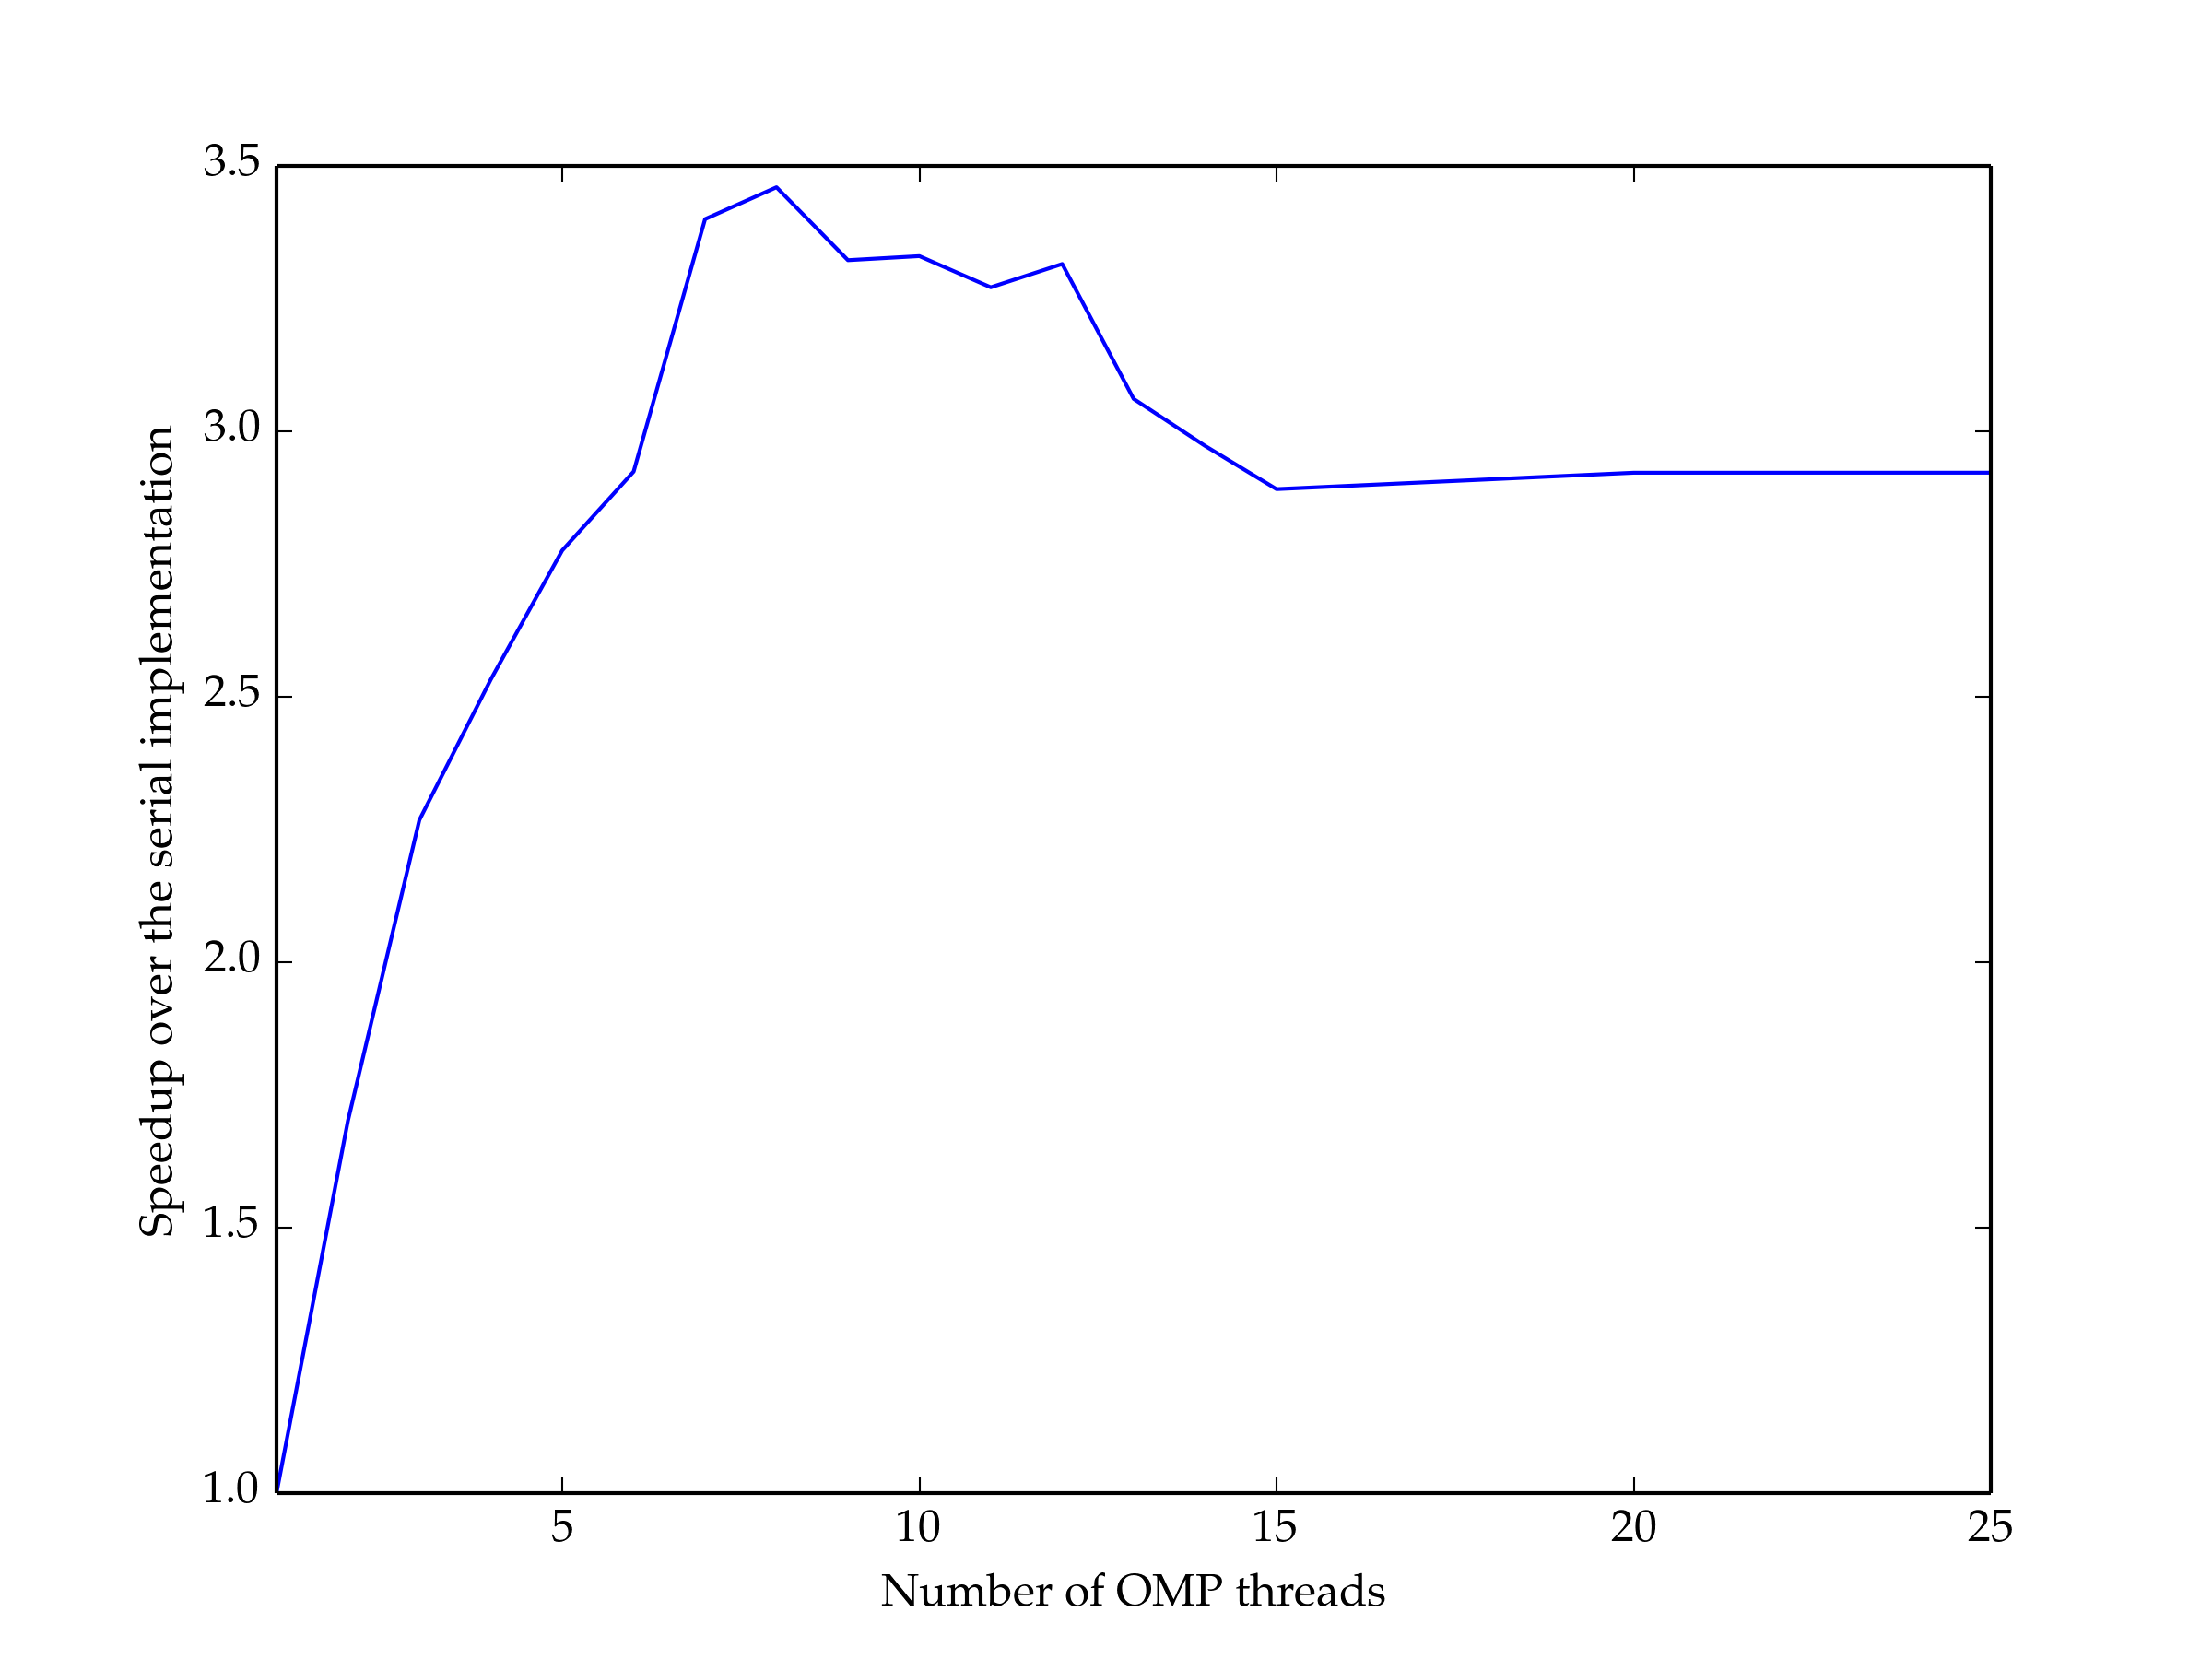
\includegraphics[width=0.9\textwidth]{./strong_scaling/strong_scaling.png}
    \caption{Speedup as a function of the number of threads}
    \label{fig:strong_scaling}
\end{figure} 


\subsubsection{Weak Scaling Study}

We vary the threads but keep the problem size/thread constant.
\begin{figure}[H]
    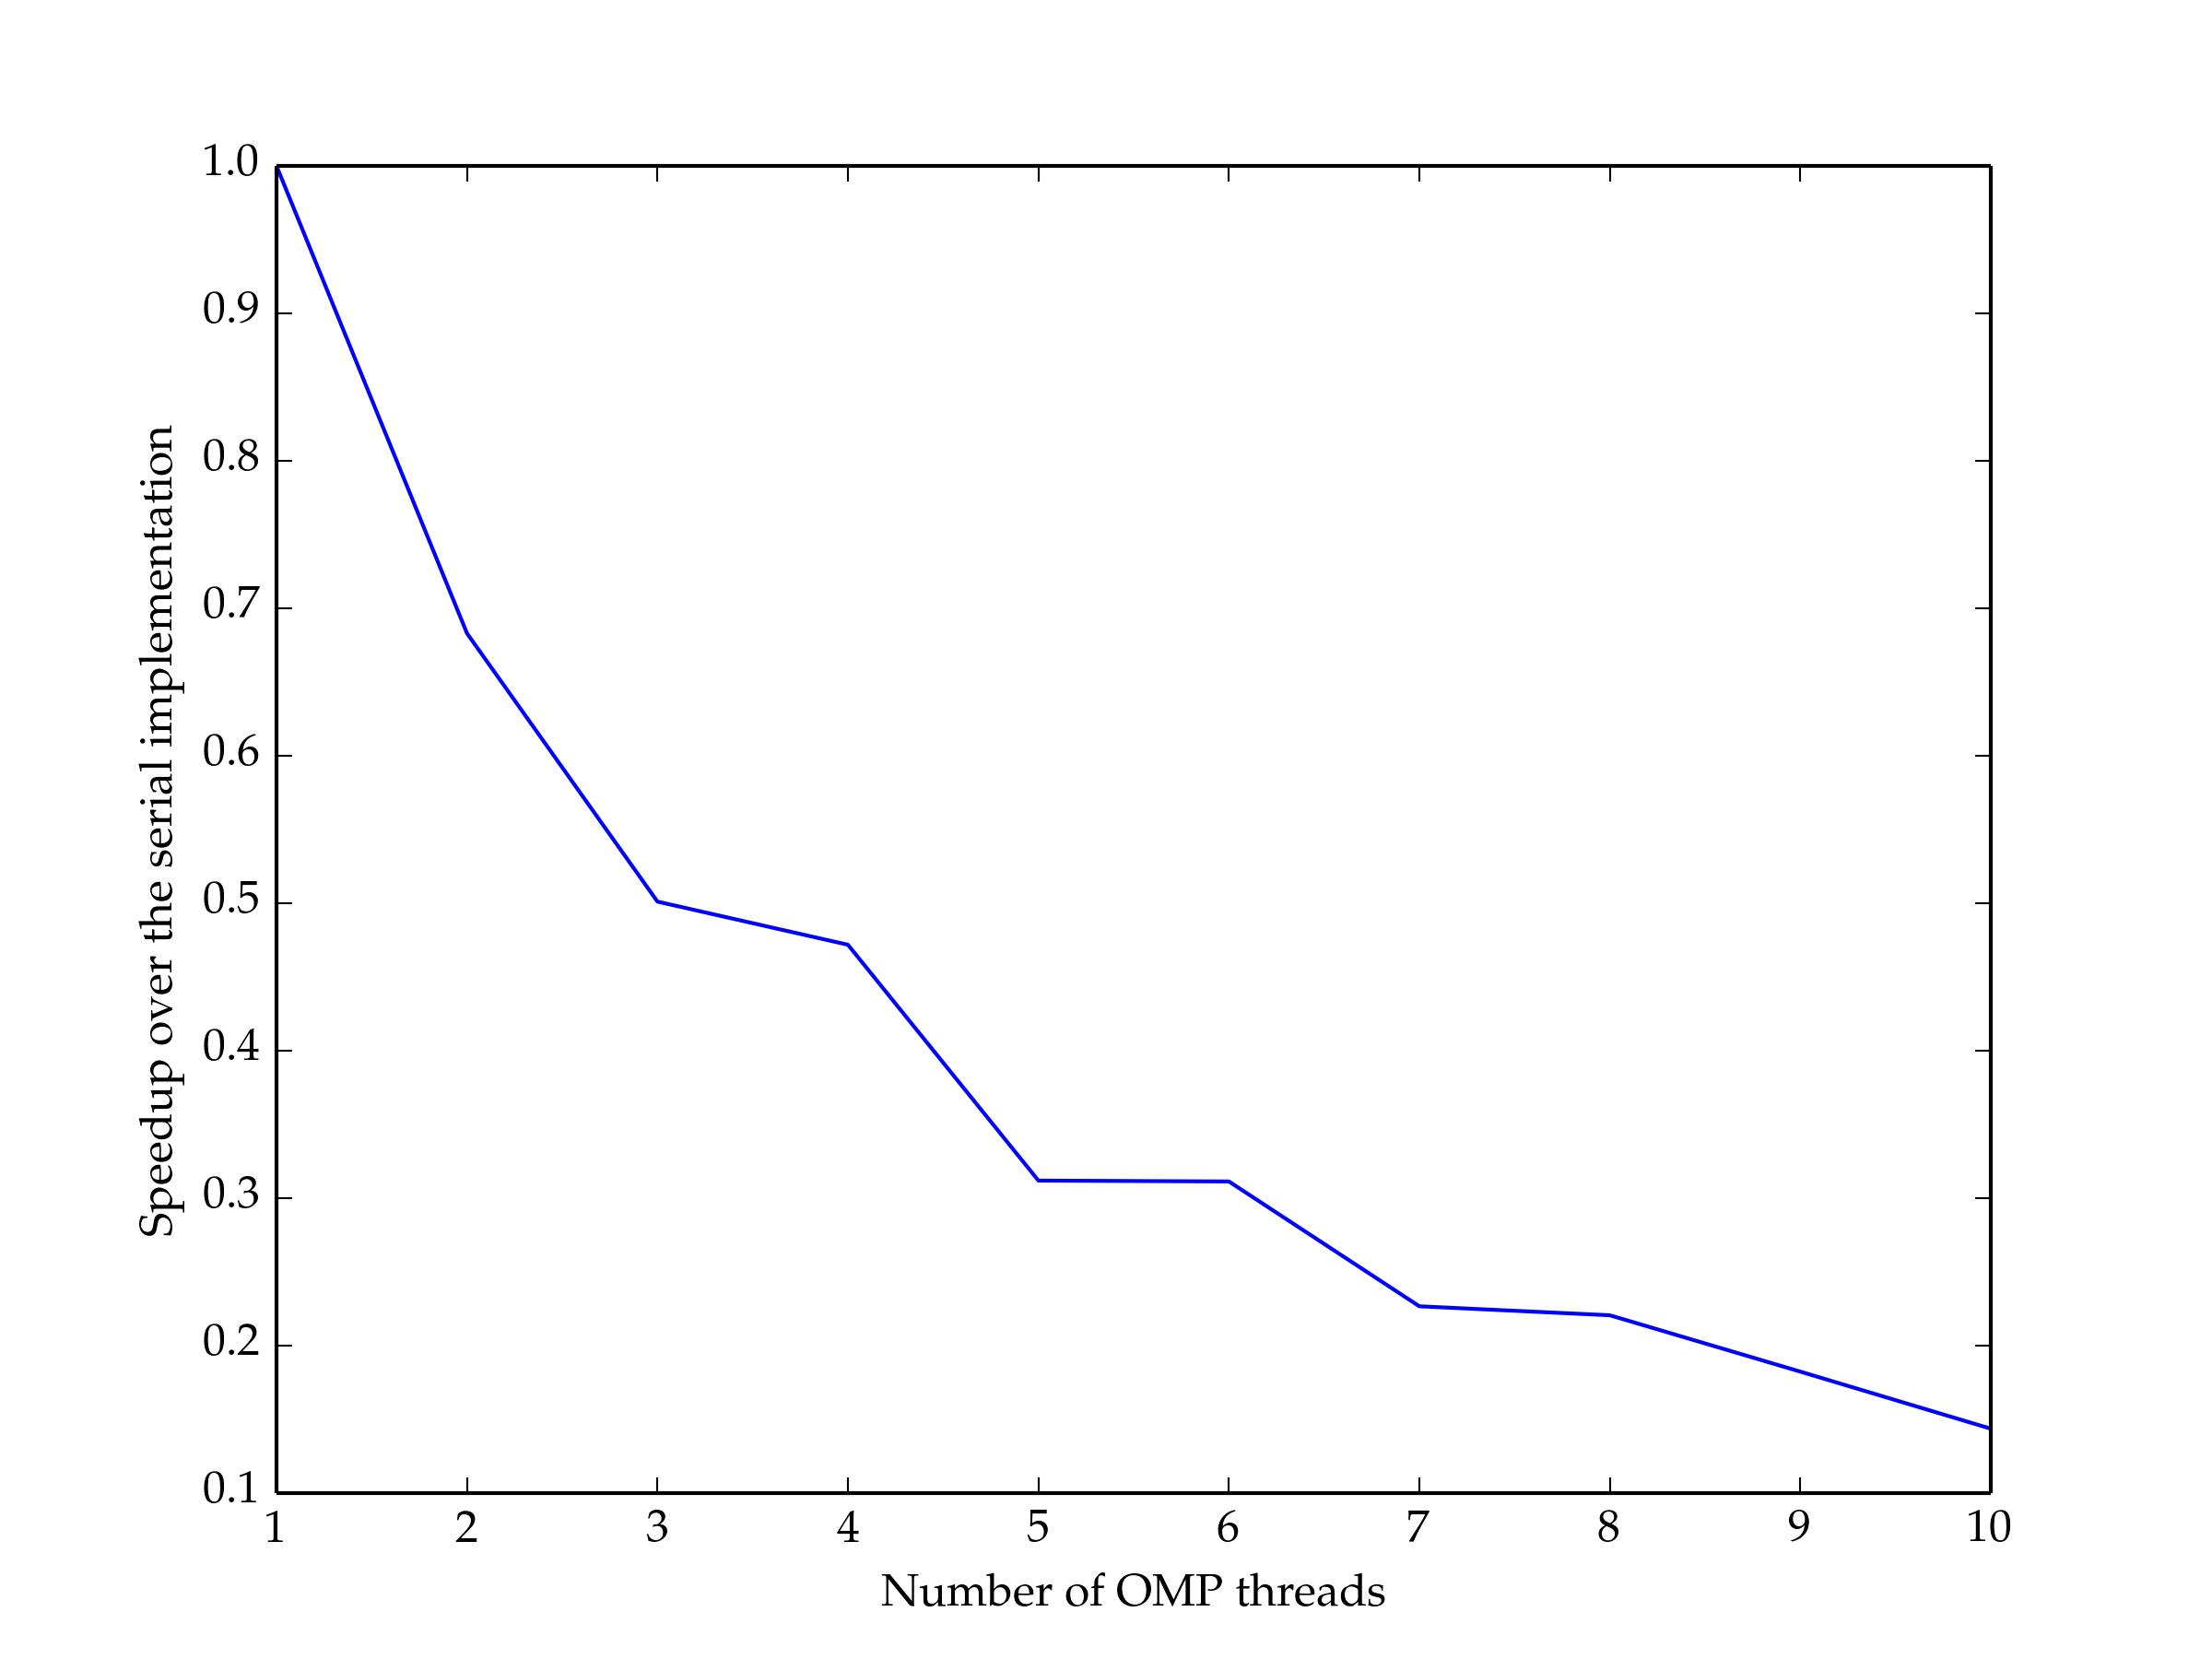
\includegraphics[width=0.9\textwidth]{./weak_scaling/weak_scaling.png}
    \caption{Speedup as a function of the number of threads}
    \label{fig:weak_scaling}
\end{figure} 



\begin{thebibliography}{9}
\bibitem{vectorization} 
Data Alignment to Assist Vectorization. (n.d.). Retrieved September 30, 2015, from \url{https://software.intel.com/en-us/articles/data-alignment-to-assist-vectorization}

\end{thebibliography}

 
 
\end{document}
